%!TEX root = ../main.tex
\chapter{Design}

\begin{figure}[t]
	\centering
	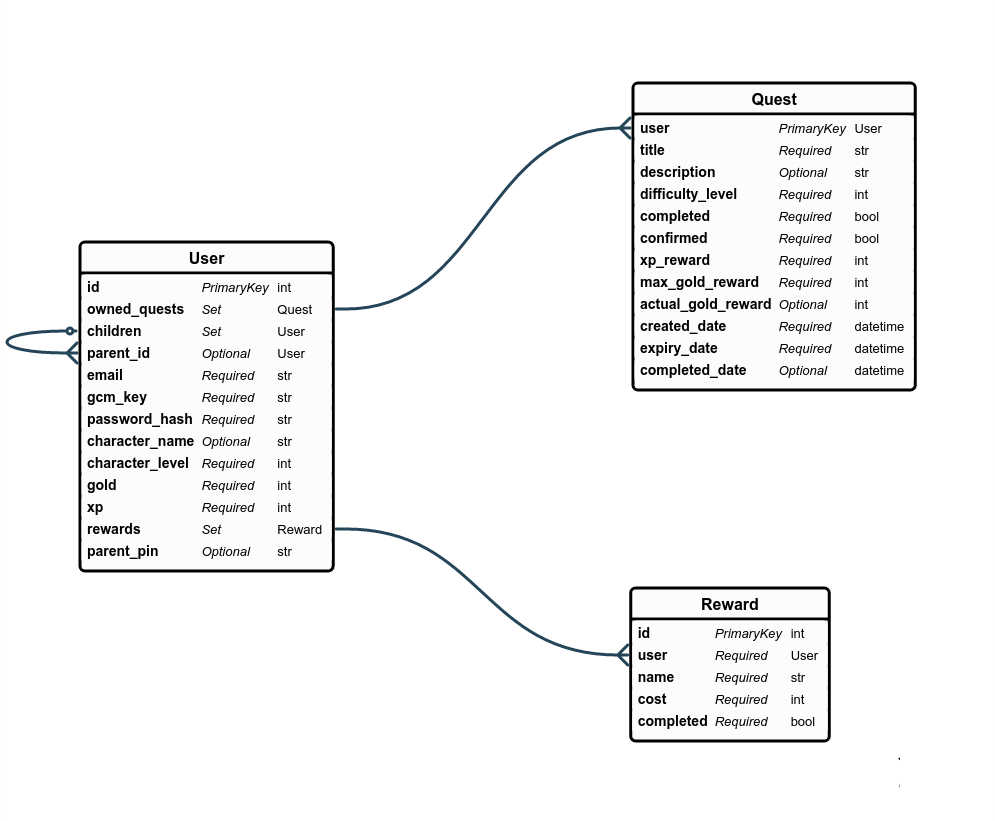
\includegraphics[width=0.45\textwidth]{images/entityRelationshipDiagram.png}
	\caption{Entity-Relationship Diagram}
	\label{fig:ERD}
\end{figure}

I chose to use a pre-built Object Relational Mapping library to interface with the database, rather than crafting particular queries on an ad hoc basis.
This was primarily for more ease-of-use purposes than any performance reasons. 
I considered a variety of options for which library to use, initially deciding upon SugarORM due to its very quick learning curve and low use of boilerplate syntax. 
However, ultimately I decided to go with GreenDAO \citep{greendao} due to more community support - based on GreenDAO having four times the number of community questions on Stack Overflow - and better documentation.

GreenDAO allowed for me 

To safely store and version control the code, I used a GitHub private repository to host my code in cloud storage and allow for me to better manage changes to the codebase.

